% Case Description: Noice
% deployment setup diagram
\begin{figure*}[b]
\centering
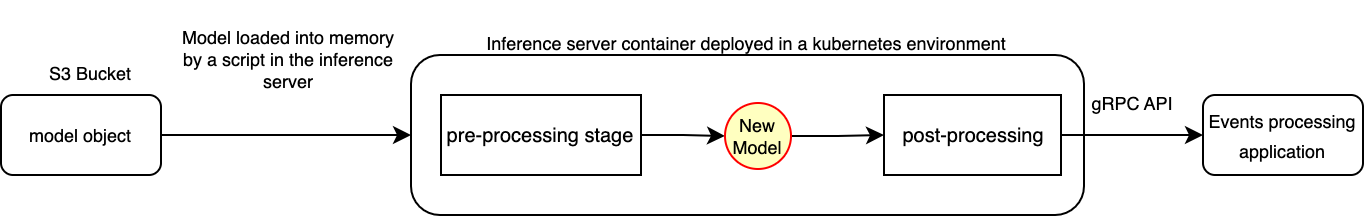
\includegraphics[width=\linewidth]{images/case2_deployment_process.png}
\caption{Case 2 Inference Architecture}
\label{fig: case2_deployment_process}
\end{figure*}

%Case Description: Smartly HLK
%deployment setup diagram
% \begin{figure*}[t]
% \centering
% 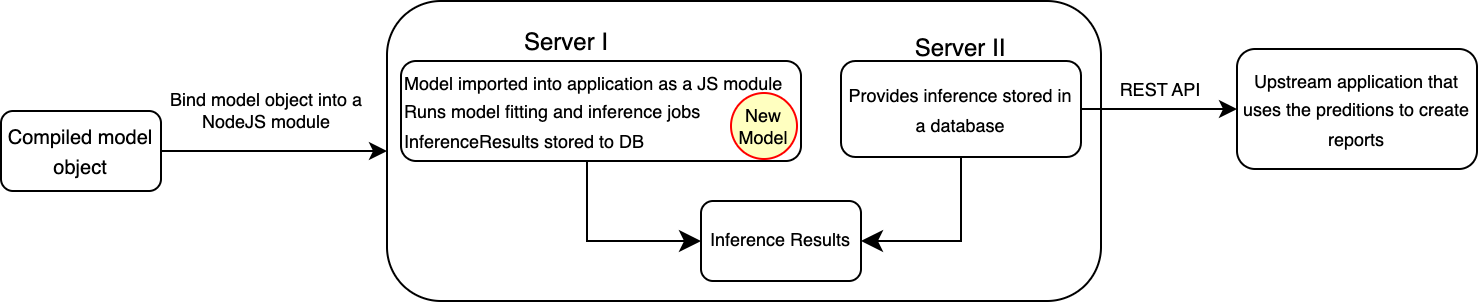
\includegraphics[width=\linewidth]{images/case1_deployment_process.png}
% \caption{Case 1 Inference Architecture}
% \label{fig: case1_deployment_process}
% \end{figure*}

This ML system is a streaming application used to process video streams. The ML system contains a pipeline of two models; an object detection model and an optical character recognition (OCR) model used to process scenes in the video stream. Prediction results from these models are integrated into a solution that seeks to enhance viewer engagement. The system takes a video stream as input data and outputs predicted labels for detected objects and text from video scenes. The solution serves real-time inference to upstream applications that rely on events in the video stream.

\textit{Pre-integration}: The trained models, prepared for deployment, are stored in binary form within an AWS S3 bucket in a designated production folder. The models are manually versioned and typically updated 1-2 times per week, with updates occurring when a newly trained model demonstrates improved offline metrics or new features are added.

\textit{Quality Assurance}: The readiness of a model is assessed through validation using a testing dataset. This involves evaluating several performance aspects of the solution, including collecting performance metrics such as F1 scores, precision, and recall, and testing the real-time inference capability to ensure that predicted events are relevant to the scenes in the video stream.

\textit{Server environment}: The binary files of the two models are loaded into a Docker container. In addition, the preprocessing and postprocessing tasks are encapsulated as functions within a script located in the container containing the model binary. Essentially, the container includes the entire inference pipeline. The model objects are directly accessed within the container, and inference is conducted by loading the loaded model object in memory through a Python script. GPUs are used for the inference process. The predictions are packaged into events as a postprocessing step of the inference procedure using a gRPC-based service for serving prediction results. The Docker images are deployed in a Kubernetes environment, enabling horizontal scaling of the system by running each new video stream in an independent container. % containers are like compute nodes

\textit{Inference}: The video data stream serves as the input to the system, where its frames are periodically sampled for predictions by the model. The inference pipeline involves three steps: (i) a preprocessing step where the frames are resized before being sent to the model for prediction, (ii) a prediction step where the resized frames are supplied to the model for inference, and (iii) a postprocessing step that packages the prediction results into a JSON format which other upstream applications can process. This inference setup is shown in Figure~\ref{fig: case2_deployment_process}. In the prediction step, the model object is accessed directly without using any communication protocol to obtain the predictions. After the postprocessing step, the overall results are served through a gRPC message service.

\textit{Monitoring}:
Monitoring is considered an online activity at the model and business levels. The model level monitoring involves tracking model accuracy using precision, recall, and F1 metrics. Business-level metrics that focus on events in a stream being correctly identified are closely related to the model-level events. The business depends on identifying these events. % The revenue model could be related to the correct identification of events to place Ads

